\section{Conclusion and Ideas:}
\begin{frame}
    \frametitle{Conclusion and Ideas:}

    \colorbox{orange}{Conclusions:}
    \begin{itemize}
        \item The ML application in wild fire is following after the framework
            the standalone ML models.
        \item The work associated with the predictive problem (e.g., predicted 
            fire behavior) or prescriptive analytics (e.g. optimizing fire
            management decisions) has relatively less number than that in other
            problem domains.
        \item In terms of vehicles, multicopters seem to be the most suitable
            for such applications
    \end{itemize}
    \colorbox{orange}{Ideas:}
    \begin{itemize}
        \item The drones can combine with the more wild fire science
            tightly, not only act as a platform to load the equipments. In other
            words, the application such as `control and navigation applications
            in the wild fire can be developed.`
        \item 3 (or even more) scales should be used to classify the researches
            in the wild fire:
            \begin{itemize}
                \item Large scale: Fire line, fire moving direction etc.
                \item Middle scale: fire zone, fire rough location.
                \item Small scale: Detailed fire map.
            \end{itemize}
    \end{itemize}

\end{frame}

%4
\begin{frame}
    \frametitle{Conclusion and Ideas:}
    \textbf{Combine the wildfire application with UAVs and Drones advantages: High
    Flexibility$\rightarrow$Diving into forest.}
    \begin{figure}[H]
        \centering
        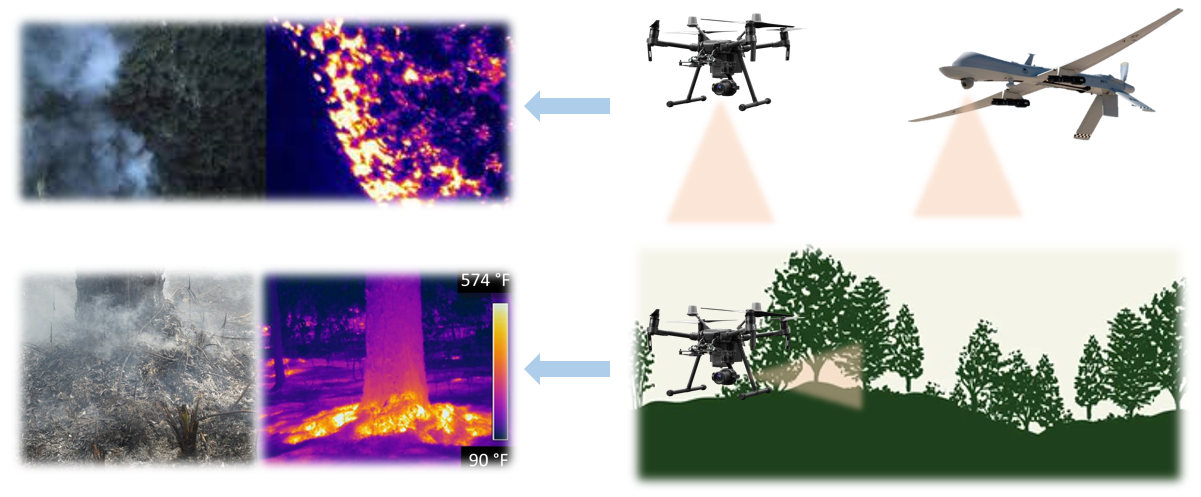
\includegraphics[width=0.6\textwidth]{./imgs/high_low.png}
        \caption{different missions according to the altitude}
        \label{1}
    \end{figure}
    \colorbox{orange}{Ideas:}
    \begin{itemize}
        \item Thermal, LiDAR and vision-based navigation method for wildfire UAVs
        \item Detection and Mapping:
            \begin{itemize}
                \item Smoldering detecting and mapping
                \item Thermal-aided SLAM for wildfire
            \end{itemize}
        \item Prediction:
            Estimate the wind direction and strength from the \textbf{smoke}
        \item Management:
            Path planning for the fireman and fire robots.
    \end{itemize}


\end{frame}
